\chapter{Úvod}
Problém existence rovinného klastrového nakreslení grafu (dále jen klastrová rovinnost) je jedním možným zobecněním klasické grafové rovinnosti pro případ, kdy kromě vrcholů a hran máme hierarchii skupin vrcholů. Skupinu vrcholů nazýváme klastrem. Pro klastrovou rovinnost není znám polynomiální algoritmus, a není známo, zda je tento problém NP-úplný. 

\begin{defn}
Mějme graf $G=(V,H)$. Pod \textit{klastrem} $C$ budeme uvažovat podmnožinu vrcholů  $C \subseteq V$. \\
\textit{Klastrovou hierarchií} jest množina klastrů, kde pro každé dva klastry $C_1$ a $C_2$ platí následující
\begin{itemize}
\item buď $C_1 \cap C_2 = \emptyset$
\item nebo $C_1 \subset C_2$
\end{itemize}
\textit{Klastrový graf} je dvojice $(G,\mathcal C)$, kde $G$ je graf a $\mathcal C$ je klastrová hierarchie.
\end{defn}

Formálně se můžeme dívat na klastrovou hierarchii jako podmnožinu $\mathcal P (V)$. To může vést k tomu, že bychom si mohli myslet, že klastrů může být velmi mnoho vzhledem k velikosti původního grafu. V kapitole složitost ukážeme, že počet klastrů je lineární vzhledem k počtu vrcholů grafu G. V některých situacích se hodí předpokládat, že množina všech vrcholů vždy tvoří klastr a též jednotlivé vrcholy tvoří klastry. Například se tento předpoklad  hodí v důkazu o počtu klastrů.

\begin{defn}
Pod \textit{klastrovým nakreslením} rozumíme to, že vrcholy a hrany nakreslíme do roviny jako u rovinného nakreslení a navíc doplníme nakreslení klastrů.\\ \textit{Nakreslením klastru} v rovině je topologická kružnice. Ve vnitřku kružnice leží pouze vrcholy z daného klastru a hrany grafu smí protínat hranici nakreslení klastru nejvýše jedenkrát. Pro libovolné dva klastry se nesmí stát, že by se jejich nakreslení protínala. Nakreslení klastru K budeme značít $\gamma_K$ \\
Klastrový graf $(G,\mathcal C)$ je \textit{klastrově rovinný} pokud existuje nějaké jeho klastrové nakreslení.
\end{defn}

Omezení pro hrany v nakreslení klastru nám zaručuje, že hrany vedoucí mezi vrcholy klastru leží celé ve vnitřku nakreslení klastru.  Podobně hrany spojující vrcholy mimo klastr musí ležet ve vnějšku. Hrana protínající nakreslenou kružnici tedy musí spojovat vrchol z klastru s vrcholem mimo klastr.

Nyní můžeme úvest definici rozhodovacího problému klastrové rovinnosti. Klastrová rovinnost má dvě základní verze. A to nakreslená a nenakreslená verze.
\begin{defn}
V \textit{nenakreslené verze klastrové rovinnosti} máme rozhodnout zda pro daný klastrový graf existuje jeho klastrové nakreslení.
\\
U \textit{nakreslené verze klastrové rovinnosti} máme na vstupu nakreslení grafu a klastrovou hierarchii a máme rozhodnout zda lze dokreslit klastry, tak abychom obdrželi klastrové nakreslení.
\end{defn}

Nakreslená verze klastrové rovinnosti je už na pohled omezena silnější podmínkou a to nakreslením vstupního grafu. Pokud tedy nelze dokreslit klastry tak, abychom obdrželi klastrové nakreslení, pak klastrový graf stále může být klastrově rovinný. Viz následující příklad 

\begin{figure}[H]
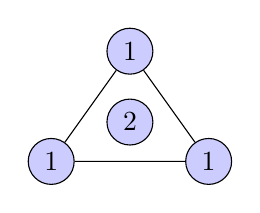
\begin{tikzpicture}[main_node/.style={circle,fill=blue!20,draw,minimum size=1em,inner sep=3pt]}]

    \node[main_node] (1) at (0,0) {1};
    \node[main_node] (2) at (-1, -1.4)  {1};
    \node[main_node] (3) at (1, -1.4) {1};
    \node[main_node] (4) at (0,-0.9) {2};

    \draw (1) -- (2) -- (3) -- (1);
\end{tikzpicture}
\caption{Čísla označují, do jakého klastru vrchol patří. Na první pohled je zřejmé, že není možné dokreslit klastr 1 tak, aby vrchol označený jako 2 nebyl ve vnitřku nakreslení klastru, ale je také zjevné, že příslušný klastrový graf je klastrově rovinný.}
\label{fig:obr1}
\end{figure}

Nyní definujeme několik pojmů, které jsou potřeba pro uvedení věty dávající kombinatorický pohled na problém klastrové rovinnosti. 

\begin{defn}
Mějme klastrový graf $(G[V,E],\mathcal C)$. Klastr K je \textit{souvislý} pokud graf indukovaný na vrcholech klastru je souvislý. 
\end{defn}

\begin{defn}
Mějme klastrový graf $(G[V,E],\mathcal C)$. \textit{Saturátor} $S$ je podmnožina ${V \choose 2} \setminus E$ taková, že každý klastr je v $(G[V,E \cup S],\mathcal C)$ souvislý. \\
Mejmě nakreslení grafu $G$, označme jej $\rho$. \textit{Nakreslený saturátor} S je množina nakreslených hran takových, že v nakreslení $\rho \cup S$ je každý každý klastr souvislý. 
\end{defn}

\begin{defn}
Mějme klastrový graf $(G[V,E],\mathcal C)$.V nakreslení klastrového grafu rozumíme \textit{dírou} kružnici v grafu ležící v klastru $K$ takovou, že v nakreslení $\gamma_K$  je uvnitř nakreslení kružnice vrchol nepatřící do klastru $K$.
\end{defn}

Větu uvedeme zvlášť pro nakreslenou verzi  a zvlášť pro nenakreslenou verzi.

\begin{theorem}Mějme nakreslenou verzi klastrové rovinnosti. Nakreslený klastrový graf $(G,\mathcal C)$ je klastrově rovinný právě tehdy, když existuje nakreslený saturátor $S$ takový, že $(G \cup S,\mathcal C)$ nemá díru.
\end{theorem}

\begin{theorem}Mějmene nakreslenou verzi klastrové rovinnosti. Klastrový graf $(G,\mathcal C)$ je klastrově rovinný právě tehdy, když existuje saturátor $S$ takový, že $G \cup S$ má rovinné nakreslení, v němž není díra vzhledem k $(G \cup S,\mathcal C)$.
\end{theorem}

\section{Aplikace klastrové rovinnosti}
Klastrová rovinnost nachází aplikaci například při vizualizace různých sítí, grafů, apod., kde je potřeba seskupovat uzly (vrcholy, ...) do celků.
